\documentclass[conference]{IEEEtran}
\usepackage{amsmath,amsfonts,amssymb}
\usepackage{graphicx}
\usepackage{listing}
\usepackage{subfig}
\usepackage{color}
\usepackage{url}
\usepackage{blkarray}
%\usepackage{url}

\begin{document}
\title{CS8803-O03 Reinforcement learning\\Project 3 report}

\author{\IEEEauthorblockN{Rohan D. Kekatpure}
\IEEEauthorblockA{Email: rdk@gatech.edu}}
% make the title area
\maketitle

% As a general rule, do not put math, special symbols or citations
% in the abstract
%\begin{abstract}
%\end{abstract}

\IEEEpeerreviewmaketitle
\section{Introduction}
Multi-agent $Q$-learning is a nontrivial departure from deterministic action, single $Q$ function MDPs. The Greenwald paper \cite{greenwald} (1) demonstrates that optimal policies in multi-agent systems could be stochastic, (2) formulates the ``correlated $Q$ learning'' algorithm to find the stochastic optimal policies and (3) shows a way to circumvent the NP-hard Nash equilibrium problem. In Project 3, we aim to reproduce Greenwald's results for a $2\times4$ grid game called ``soccer''.
%%
\section{Quick theory tour}
The paper presents four multi-agent $Q$ learning options:
\begin{enumerate}
\item {\bf $Q$ learning:} Ignores the opponent's $Q$ function and actions. Agents are coupled only through rewards. The policy is deterministic and $Q$ function at each state for each agent is a vector of $n$ values ($n=5$). The state value for agent $i$ is max over the $Q$ vector: 
\begin{equation}
V_i =\max_{a\in A_i} Q_i(s,a)
\end{equation} 
%
\item {\bf Friend $Q$: } Ignores the opponent's $Q$ function, but works with joint action space. Optimal policy is deterministic, and $Q$ function at each stage for each agent is a $n\times n$ matrix. The state value for agent $i$ is the max over the $Q$ matrix:
\begin{equation}
V_i = \max_{\vec{a}\in A_1\times A_2} Q_i(s, \vec{a})
\end{equation}
%
\item {\bf Foe $Q$: } Ignores opponent's $Q$ function, but calculates the value using {\bf maximin} instead of  max and requires linear programming (LP). Maximin also allows {\bf stochastic} optimal policies represented as a probability distribution over $n$ action values. The $Q$ function at each state for each agent is an $n\times n$ matrix and the state value is given by: 
%
\begin{equation}
V_i = \max_{\pi\in\text{PD}(A)}\min_{o\in O}\sum_{a\in A_i}\pi(a) Q_i(s, a, o)
\end{equation}
%
\item {\bf CE $Q$: } Considers opponent's Q as well as joint actions and computes state value as a function as:
%
\begin{equation}
V_i = \sum_{\vec{a}\in A_1\times A_2} \sigma(\vec{a})Q_i(s, \vec{a})
\end{equation}
where $\sigma(\vec{a})$ is a probability distribution over the $n^2$ action pairs $\vec{a}$ computed using the {\em u}CE-Q objective out of the four CE options provided. In simplified notation:
\begin{equation}
\sigma = \arg \max_{\sigma\in\text{CE}} \sum_{\vec{a}\in A_1 \times A_2} \sigma(\vec{a})\big[Q_1(s, \vec{a}) + Q_2(s, \vec{a})\big]
\end{equation}
\end{enumerate}
%%
\section{Implementation}
\subsection{Game representation}
The soccer world is a $2\times 4$ grid with row index $r\in [1,2]$ and column index $c\in [1,2,3,4]$. The state of the game is represented as:
\begin{equation}
s \stackrel{\Delta}{=} \text{tuple}((r_A,c_A), (r_B,c_B), \text{ball})
\end{equation}
The individual action space is $A_1, A_2 \in [N, W, E, S, T]$ ($T=$ stick) and the joint action space is $A_1\times A_2$. Since the number of states $ = 8\times 7\times 2 = 112$ is small, the $Q$ values can be maintained in memory as a nested dictionary:
\begin{equation}
Q \stackrel{\Delta}{=} \{s: \{\vec{a}: (v_A, v_B)\}\} 
\end{equation}
where the inner dictionary maps 25 action pairs to a tuple of $Q$ values for agents $A$ and $B$, and the outer dictionary maps this structure to the state. The structure can also be thought as a mapping from each of the 112 states to a $5\times 5\times 2$ (or $5\times 1\times 2$ for $Q$ learning) matrix of $Q$ values for agents $A$ and $B$ for each action pair. 
%%
\subsection{Simulation}
A {\bf move} is defined as one action each by $A$ and $B$ carried out in a random order. An {\bf episode} is a set of moves until a goal is scored. An episode can: (1) in theory continue forever and (2) end mid-move if a goal is scored.

To simulate a move, we select an action pair $(a_1, a_2)$ from $A_1\times A_2$ and assign it to $(A, B)$, who execute in random order. After executing its assigned action, each agent checks for the game-end condition and receives rewards for reaching the next state. Rewards are zero except when a goal is scored. In addition to the prescribed rules, we observed the following additional conventions: (1) an episode never starts in the end condition, (2) goal is counted even when a stationary empty-handed agent in a goal position is handed a ball by the mobile ball-carrying agent; i.e. $A$ could lose if it is in $B$'s goal position and handed a ball.

After each move, values $V_i$, $i\in [A,B]$ for each state are calculated and used to update the two $Q$-functions according to the update equations in Table 1 in \cite{greenwald}:
%%
\begin{equation}
Q_i^{t+1}(s, a) \leftarrow (1-\alpha_t) Q_i^t(s, a) + \alpha_t\big[(1-\gamma) R_i^t + \gamma V_i^t(s)\big]
\end{equation}
%%
where the action variable $a$ is a single action in case of $Q$-learning and Foe $Q$ and an action vector, $\vec{a}$, for Friend $Q$ and CE $Q$. Because of the small number of states, we learn via an {\bf off-policy} $Q$ learning algorithm (i.e. actions are always random).
%%
%%
\begin{figure*}[tbp]
\centering 
\begin{tabular}{cc}
    \subfloat[CE-Q] {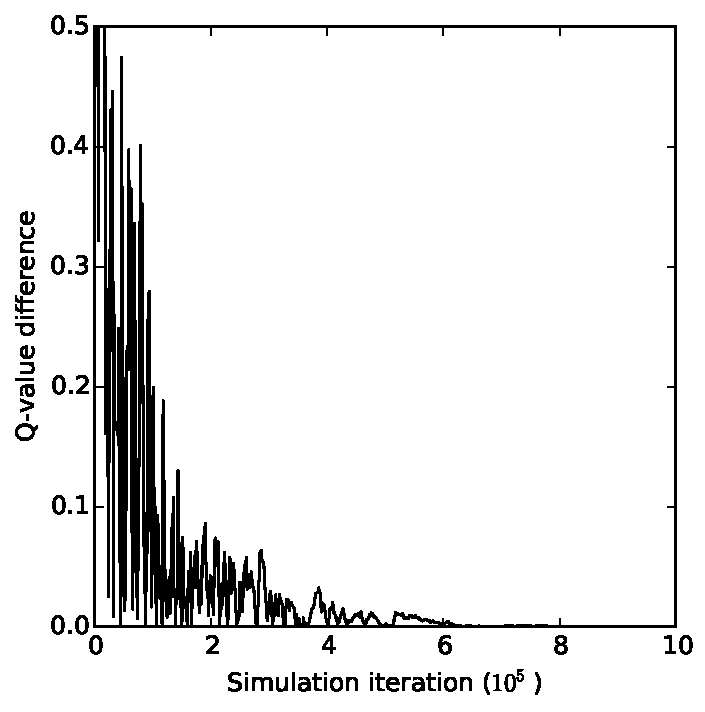
\includegraphics[width=0.4\textwidth]{./figures/ceq.pdf}} 
    & \subfloat[Foe-Q] {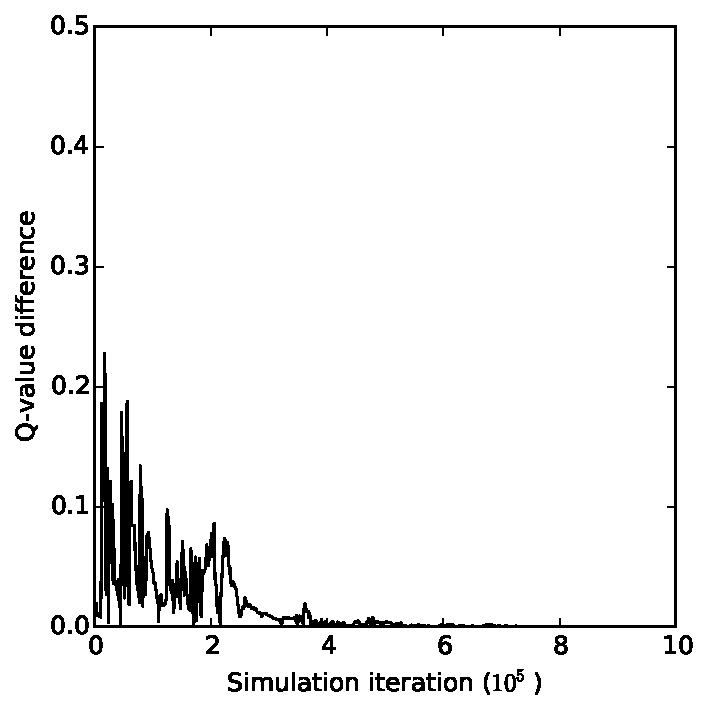
\includegraphics[width=0.4\textwidth]{./figures/foe.pdf}} \\
    \subfloat[Friend-Q] {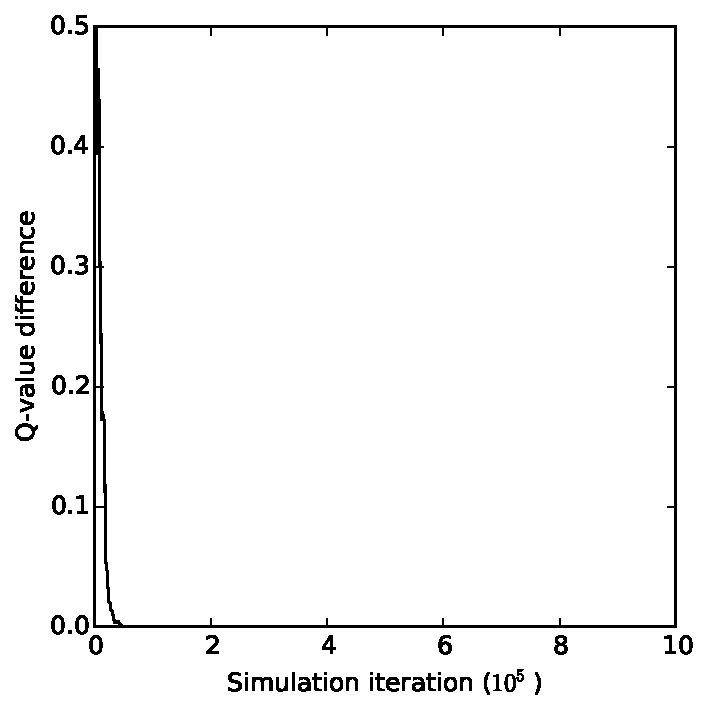
\includegraphics[width=0.4\textwidth]{./figures/friend.pdf}}
    & \subfloat[Q-learning] {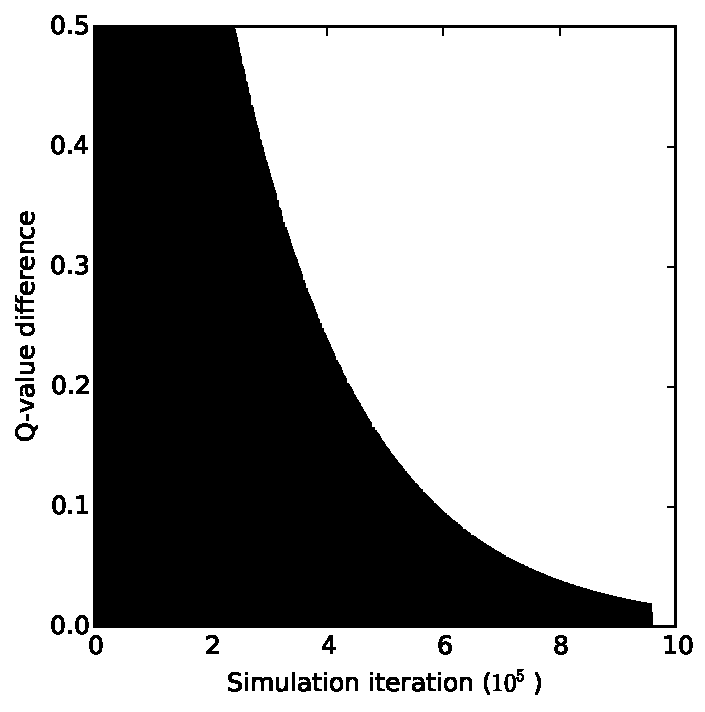
\includegraphics[width=0.4\textwidth]{./figures/qlearning.pdf}}    
\end{tabular}
\caption{Results of the soccer game in the Greenwald paper. (a) Correlated $Q$, (b) Foe $Q$, (c) Friend $Q$ and (d) $Q$ learning.\label{fig:maql}}
\end{figure*}
%%
\subsection{Recording $Q$-function difference}
The paper reports the evolution of the $Q_A$ values for the state $s = ((1, 3)_A,(1,2)_B, B)$ (a.k.a the monitor state) for the action pair $\vec{a} = ST$. The evolution of the $Q$ values for the monitor state are stored in an array and updated only when that state is actually encountered in an episode. A global timestep counter, which increments across episodes, is maintained to record the value of the timesteps at which the monitor state is updated. The $Q$-function difference is calculated exactly according to the prescription: $\textsc{err}_A^t = \vert Q_A^t(s, \vec{a}) - Q_A^{t-1}(s, \vec{a})\vert$.
\subsection{Linear programming}
Correlated Q and Foe Q implementation require LP. After some research \cite{cvxopt}, we chose the {\tt CVXOPT} LP package with the GNU {\tt glpk} solver. This resulted in over $10\times$ speedup relative to {\tt PuLP}, {\tt SciPy} and {\tt CVXOPT}'s default solver. However, setting up the problem in {\tt CVXOPT}'s matrix language requires care (proper negations, column ordering etc).
\subsection{Software dependencies}
The only external packages for our implementation are {\tt CVXOPT}, {\tt numpy} for core computation and {\tt matplotlib} and {\tt Pandas} for postprocessing.
\subsection{Hyperparameters}
We experienced that the convergence curves are {\bf sensitive} to the choice of initial learning rate and the decay schedule. The converged values are less sensitive. We've collected the hyperparemeters of our implementation in Table~\ref{tab:hyper}.
\begin{table}[!h]
\begin{center}
\begin{tabular}{|l|l|}
\hline
Hyperparameter & Value\\ \hline 
Discount $\gamma$ & 0.9\\
Decay schedule & $\alpha = \max(\alpha_{\text{min}}, \alpha_0\alpha_d^t$) \\
$\alpha_0$ & 0.15 \\
$\alpha_{\text{min}}$ & $10^{-3}$ \\ 
$\alpha_d$ & 0.9999954 \\ \hline
\end{tabular}
\end{center}
\caption{Hyperparameters for all $Q$-learning algorithms. \label{tab:hyper}}
\end{table}
%%
\section{Results}
Before discussing the actual results, note that the {\bf spirit} of the assignment is (1) to demonstrate that regular and Friend $Q$ learning do not work in stochastic multi-agent situations and (2) to discover stochastic optimal policies for multi-agent environments. While we aim to reproduce Greenwald results, we don't try to eliminate small cosmetic differences, as long as optimal policies match.

The results of the simulation of the soccer game are displayed in Fig.~\ref{fig:maql} and are in the same order as \cite{greenwald}. Below is a summary of results:
%
\begin{enumerate}
\item Regular $Q$-learning, shown in Fig.~\ref{fig:maql}(d), does not converge, but instead simply traces the decay schedule. The trend of our $Q$-learning curve and the general conclusion is consistent with \cite{greenwald}.
%
\item Friend $Q$ shown in Fig.~\ref{fig:maql}(c) converges, but it converges to a deterministic action  by design (i.e. Friend $Q$ algorithm doesn't seek a probability distribution). Our results converge at $\sim50000$ timesteps, which is close to what can be estimated from the paper. 
%
\item Foe $Q$, shown in Fig.~\ref{fig:maql}(b) allows for stochastic actions by computing probability distribution over {\em independent} action vectors. The Foe $Q$ probability distribution for $A$ and $B$ converge to
%
\begin{align*}
\pi_A &= (0.00, 0.00, 0.00, 0.32, 0.68)\\
\pi_B &= (0.00, 0.00, 0.00, 0.68, 0.32)
\end{align*}
%
for actions $[N, W, E, S, T]$ respectively. So The agent is randomizing between sticking and heading south. Intuitively equilibrium values ought to be 0.50. Any {\bf asymmetry} in the agents' stochasticity exposes it to exploitation by opponent: if $B$ knows $A$ leans toward heading south, it can increase its reward by {\bf biasing} toward sticking. We were unable to investigate this further due to time constraints.
%
\item Correlated $Q$ results are plotted in Fig.~\ref{fig:maql}(a). The graph appears similar to the paper. The converged joint action probability distribution, $\sigma(\vec{a})$ is:
\begin{equation*}
\sigma(\vec{a}) = 
\begin{blockarray}{cccccc}
&N & W & E & S & T \\
\begin{block}{c(ccccc)}
  N & 0.00 & 0.00 & 0.00 & 0.00 & 0.00 \\
  W & 0.00 & 0.00 & 0.00 & 0.00 & 0.00 \\
  E & 0.00 & 0.00 & 0.00 & 0.00 & 0.00 \\
  S & 0.00 & 0.00 & 0.00 & {\color{blue}0.30} & {\color{blue}0.30} \\
  T & 0.00 & 0.00 & 0.00 & {\color{blue}0.22} & {\color{blue}0.18}\\
\end{block}
\end{blockarray}
\end{equation*}
which agrees with the optimal policy for Foe $Q$ that $A$ and $B$ randomize between sticking and heading south. Often the probability mass in action $T$ is concentrated in action $N$ which, given our convention, is same as $T$ when in top row. There is again an asymmetry (the rows and columns don't sum to 0.5), which we were not able to investigate due to lack of time.
\end{enumerate}
\subsection{Why are Foe and CE $Q$ curves different?}
Our graphs for Foe and CE $Q$ trainings are different while the Greenwald paper has identical graphs for these two experiments. Even if the randomizer seed is kept the same, there are reasons to expect this difference.  Foe and CE $Q$ formulations solve entirely different optimization problems. Specifically, (1) Foe $Q$ computes the action probability distribution by using maximin over {\em independent} action spaces, while {\em u}CE $Q$ probability distribution is over {\em joint} action space. (2) Foe $Q$ objective involves $Q$ function of a {\bf single} agent while the {\em u}CE $Q$ objective involves the {\bf sum} of the agent's $Q$ functions. (3) A CE $Q$ with $n$ individual actions, has $2n(n-1)$ {\bf rationality} constraints in addition to positivity and normalization. In the face of these differences, we can't see an obvious reason why the formulations would show identical $Q$ value updates.

Despite the differences in convergence, the Foe and CE $Q$ both yield {\bf identical} optimal stochastic policies. In this respect we did reproduce the results of the Greenwald paper.
%%
\section*{Summary}
We were successfully able to reproduce {\bf all  four} graphs in the paper as well as optimal stochastic policies for Friend and CE $Q$ algorithms. The small differences are due to different choices of learning rates, decay schedules and inherent stochasticity.

Without project 3, our understanding of multi-agent systems would have been superficial. Despite the seemingly simple soccer world, synthesis and implementation of the Greenwald paper has not only enhanced our theoretical understanding, but provided a deep appreciation of practical issues in coding multi-agent RL systems.
%%
\begin{thebibliography}{1}
\bibitem{greenwald}
A.~Greenwald and K.~Hall, ``Correlated Q learning,'' {\em ICML}, 2001.
\bibitem{cvxopt}
S.~Caron,``Linear Programming in Python with CVXOPT,'' {\em \url {https://scaron.info/blog/linear-programming-in-python-with-cvxopt.html}}
\end{thebibliography}

\end{document}


